\documentclass{ceurart}
\sloppy
\usepackage{listings}
\lstset{breaklines=true}
\usepackage{booktabs}
\usepackage{multirow}
\usepackage{tabularx}
\usepackage{float}
\usepackage{amsmath}
\usepackage{pgfplots}
\usepackage{tikz}
\usetikzlibrary{shapes,arrows,positioning,fit,backgrounds,calc}
\pgfplotsset{compat=1.18}
\usepackage{eso-pic}
\usepackage{transparent}
\usepackage{xcolor}

\definecolor{iitblue}{RGB}{0,47,108}
\definecolor{iitgold}{RGB}{186,146,28}
\definecolor{codered}{RGB}{180,0,0}
\definecolor{codegray}{RGB}{128,128,128}

%% Watermark
\AddToShipoutPictureBG{%
  \AtPageCenter{%
    \makebox(0,0){%
      \transparent{0.06}%
      \includegraphics[width=9cm]{iit_roorkee_logo.png}%
    }%
  }%
}

\begin{document}

\copyrightyear{2026}
\copyrightclause{Copyright for this paper by its authors.
  Use permitted under Creative Commons License Attribution 4.0
  International (CC BY 4.0).}

\conference{CLEF 2026 Working Notes, 21--24 September 2026, Jena, Germany}

\title{From Frozen Encoders to Multi-Agent LLM Pipelines: An Iterative Journey through Person--Place Relation Extraction in Multilingual Historical Texts}

\title[mode=sub]{Team Hansel\&Gretel at CLEF HIPE-2026}

\author[1]{Pradyuman Singh Shekhawat}[%
  email=pradyuman_ss@cs.iitr.ac.in,
]
\cormark[1]

\author[1]{Rohan Gupta}[%
  email=rohan_g@cs.iitr.ac.in,
]

\address[1]{Indian Institute of Technology Roorkee, Roorkee, Uttarakhand 247667, India}

\cortext[1]{Corresponding author. Also reachable at: shekhawat.pradyuman10@gmail.com}

\begin{abstract}
We present the system description and experimental analysis of Team Hansel\&Gretel for the CLEF HIPE-2026 Shared Task on Person--Place Relation Extraction from Historical Multilingual Documents. The task requires classifying, for each person--location pair in a historical newspaper article (German, French, or English, spanning the 19th--20th centuries), two temporal relations: \texttt{at} (person was ever at the location, 3-class) and \texttt{isAt} (person was there within approximately one month of publication, binary). Evaluation uses Macro Recall, equally weighting all label classes. We explore nine progressively sophisticated strategies, from a frozen XLM-RoBERTa encoder with classical ML classifiers (Global Macro Recall $= 0.6018$) to a Qwen2.5-3B-Instruct Generative Supervised Fine-Tuning pipeline with Wikidata knowledge injection ($= 0.7289$) and a three-agent Historian--Geographer--Arbiter multi-agent architecture ($= 0.7280$). This paper documents the design decisions, failure modes, and key insights behind each strategy, providing a comprehensive account of iterative NLP system development under data scarcity, class imbalance, and multilingual historical OCR noise.
\end{abstract}

\begin{keywords}
  Person--Place Relation Extraction \sep
  Historical NLP \sep
  Multilingual Transformers \sep
  XLM-RoBERTa \sep
  LoRA \sep
  Generative Classification \sep
  Multi-Agent LLM \sep
  Wikidata \sep
  HIPE-2026 \sep
  CLEF
\end{keywords}

\maketitle

%%==========================================================================
\section{Introduction}
%%==========================================================================

The digitisation of historical newspapers has created vast corpora of 19th and 20th century text encoding biographical trajectories and cultural history. Automatically recovering \emph{where people were and when} from these documents enables digital humanities scholars to reconstruct spatio-temporal life trajectories at scale. This is the central challenge of \textbf{CLEF HIPE-2026}~\cite{hipe2026guidelines}: the Shared Task on Person--Place Relation Extraction from multilingual historical documents.

Unlike standard named entity recognition, HIPE-2026 requires \emph{temporal reasoning}: a system must determine whether a text provides evidence for a \emph{historical} presence (\texttt{at}) or a \emph{contemporary} one (\texttt{isAt}, bounded to $\approx$1 month before publication). This distinction, combined with multilingual OCR-noisy text, severe class imbalance, and a small labelled dataset, makes the task deceptively difficult.

Team Hansel\&Gretel approached this as an iterative research problem, developing \textbf{nine distinct strategies} that form a natural progression:

\begin{enumerate}
  \item \textbf{S1}: Frozen XLM-RoBERTa + Classical ML classifiers
  \item \textbf{S1.5}: Multi-Task Learning (MTL) + Optuna Hyperparameter Optimisation
  \item \textbf{S2}: Full End-to-End XLM-RoBERTa Fine-Tuning
  \item \textbf{S2.5}: PEFT/LoRA on XLM-RoBERTa
  \item \textbf{S3}: Monolingual LoRA Routing (language-partitioned adapters)
  \item \textbf{S4/S4.5}: Qwen2.5-0.5B MTL with LoRA (+ soft label variant)
  \item \textbf{S5}: Qwen2.5-3B-Instruct Generative SFT \emph{(best single model)}
  \item \textbf{S6/S7}: Three-specialist multi-agent pipeline (Historian/Geographer/Arbiter)
  \item \textbf{S8/S9}: Chain-of-Thought few-shot via IBM RITS large LLMs + Wikidata injection
\end{enumerate}

%%==========================================================================
\section{Task Description}
%%==========================================================================

\subsection{Formal Definition}

HIPE-2026 provides historical newspaper documents as input. Each document contains full article text with metadata (title, publication date, language) and a list of sampled (person, location) entity pairs. For each pair, systems classify two relations:

\begin{equation}
  f(\text{context}, (\text{person}, \text{location})) \mapsto \Big(\underbrace{\texttt{at}}_{\in\{\texttt{TRUE},\texttt{PROBABLE},\texttt{FALSE}\}},\ \underbrace{\texttt{isAt}}_{\in\{\texttt{TRUE},\texttt{FALSE}\}}\Big)
\end{equation}

The \textbf{\texttt{at}} relation is ternary: \texttt{TRUE} if the text explicitly places the person at the location at any past time; \texttt{PROBABLE} if inferable from implicit cues; \texttt{FALSE} otherwise. The \textbf{\texttt{isAt}} relation is binary: \texttt{TRUE} only within $\sim$1 month of publication. A hard \emph{transitivity constraint} applies: $\texttt{isAt}=\texttt{TRUE} \implies \texttt{at} \in \{\texttt{TRUE},\texttt{PROBABLE}\}$.

\subsection{Evaluation Metric}

The primary metric is \textbf{Macro Recall}, computed independently per sub-task:
\begin{equation}
  \mathrm{MacroRecall} = \frac{1}{|L|}\sum_{\ell \in L} \frac{\#\text{correctly predicted with label }\ell}{\#\text{examples with gold label }\ell}
\end{equation}
The \textbf{Global Score} averages both sub-task macro recalls. Three evaluation profiles are assessed: \textbf{Accuracy} (Macro Recall on Test A), \textbf{Efficiency} (composite rank: accuracy + parameter count + model size), and \textbf{Generalisation} (Macro Recall on surprise literary Test B, \texttt{at} only).

%%==========================================================================
\section{Dataset Analysis}
%%==========================================================================

\subsection{Data Sources and Splits}

The dataset derives from HIPE-2022~\cite{hipe2022} entity-annotated corpora, re-annotated for person--place relation extraction. It covers four historical newspaper collections (hipe2020, sonar, newseye, letemps) in German, French, and English spanning 1780--1950.

\begin{table}[ht]
  \caption{Gold dataset statistics by language split (v1.0).}
  \label{tab:data}
  \centering
  \begin{tabular}{lrrrr}
    \toprule
    \textbf{Lang.} & \textbf{Train Docs} & \textbf{Train Pairs} & \textbf{Dev Docs} & \textbf{Dev Pairs} \\
    \midrule
    German (DE)  & 97  & 1,345 & 32  & 432   \\
    French (FR)  & 328 & 4,521 & 109 & 1,557 \\
    English (EN) & 56  & 501   & 18  & 148   \\
    \midrule
    \textbf{Total} & \textbf{481} & \textbf{6,367} & \textbf{159} & \textbf{2,137} \\
    \bottomrule
  \end{tabular}
\end{table}

In addition, a \textbf{silver-labelled sandbox} corpus ($\sim$461 docs, 6,170 pairs) of automatically annotated documents provides auxiliary training signal.

\subsection{Exploratory Data Analysis (EDA)}

We performed detailed EDA on the gold training split available at experiment time (104 documents, 1,251 pairs):

\begin{table}[ht]
  \caption{Gold training split EDA statistics (104 documents).}
  \label{tab:eda}
  \centering
  \begin{tabular}{lr}
    \toprule
    \textbf{Metric} & \textbf{Value} \\
    \midrule
    Total candidate pairs & 1,251 \\
    Language split & 34 DE / 35 EN / 35 FR \\
    Unique persons & 496 \\
    Unique locations & 469 \\
    Average document length & 3,465 chars \\
    Maximum document length & 11,738 chars \\
    \texttt{at}: TRUE / PROBABLE / FALSE & 441 / 120 / 690 \\
    \texttt{isAt}: TRUE / FALSE & 279 / 972 \\
    \bottomrule
  \end{tabular}
\end{table}

Three challenges shaped all modelling decisions:

\begin{enumerate}
  \item \textbf{Context Length}: Max $\sim$12,000 chars ($\approx$3,000 tokens) exceeds standard 512-token encoder limits, motivating generative LLMs.
  \item \textbf{Class Imbalance}: \texttt{isAt=FALSE} at 77.7\%; \texttt{PROBABLE} at 9.6\% of \texttt{at} labels. Macro Recall penalises naive majority-class predictors heavily.
  \item \textbf{Multilingual by Design}: Equal DE/EN/FR split — monolingual models immediately lose cross-lingual transfer.
\end{enumerate}

\begin{figure}[ht]
  \centering
  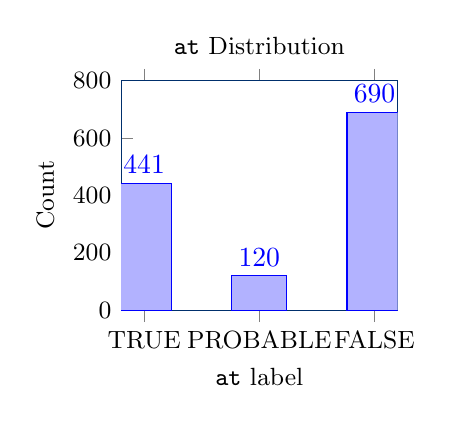
\begin{tikzpicture}
  \begin{axis}[
    ybar, width=0.42\textwidth, height=4.5cm,
    bar width=0.7cm,
    symbolic x coords={TRUE,PROBABLE,FALSE},
    xtick=data, ymin=0, ymax=800,
    ylabel={Count}, xlabel={\texttt{at} label},
    title={\texttt{at} Distribution},
    nodes near coords, nodes near coords align=vertical,
    title style={font=\small}, label style={font=\small},
    tick label style={font=\small}, fill=iitblue, draw=iitblue,
  ]
  \addplot coordinates {(TRUE,441)(PROBABLE,120)(FALSE,690)};
  \end{axis}
  \end{tikzpicture}
  \hfill
  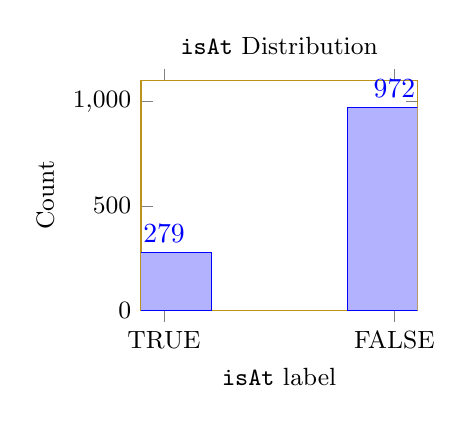
\begin{tikzpicture}
  \begin{axis}[
    ybar, width=0.42\textwidth, height=4.5cm,
    bar width=1.2cm,
    symbolic x coords={TRUE,FALSE},
    xtick=data, ymin=0, ymax=1100,
    ylabel={Count}, xlabel={\texttt{isAt} label},
    title={\texttt{isAt} Distribution},
    nodes near coords, nodes near coords align=vertical,
    title style={font=\small}, label style={font=\small},
    tick label style={font=\small}, fill=iitgold, draw=iitgold,
  ]
  \addplot coordinates {(TRUE,279)(FALSE,972)};
  \end{axis}
  \end{tikzpicture}
  \caption{Label distributions in the gold training set. Severe imbalance in \texttt{isAt} (78\% FALSE) drives the choice of Macro Recall as the evaluation metric.}
  \label{fig:labels}
\end{figure}

\subsection{Why This Dataset Is Particularly Challenging}

The HIPE-2026 data presents a unique confluence of difficulties rare in modern NLP benchmarks: (1) \textbf{OCR noise} from historical typesetting (e.g., ``Mufschen'' for ``Munchen''); (2) \textbf{archaic vocabulary} and grammar absent from modern pre-training corpora; (3) \textbf{temporal reasoning} over implicit signals (verb tense, temporal adverbs, publication dates); (4) \textbf{entity ambiguity} (same mention, different individuals); and (5) \textbf{data scarcity} ($\sim$100 gold documents across 3 languages and 3 label classes).

%%==========================================================================
\section{Organiser Baseline}
%%==========================================================================

The HIPE-2026 organisers provided a minimal LLM baseline~\cite{hipe2026baseline} using \texttt{mistralai/Ministral-3-3B-Instruct-2512} (GGUF quantised) via \texttt{llama-cpp-python}, zero-shot with greedy decoding. It reads and writes the official HIPE-2026 JSONL format.

Our random baseline experiment (via \texttt{dummy\_predict.py}) yielded: \texttt{at} MR $= 0.3211$, \texttt{isAt} MR $= 0.5273$, \textbf{Global MR $= 0.4242$}. This establishes the floor: any meaningful system must substantially exceed 0.4242.
%%==========================================================================
\section{Strategies S1 and S1.5: Frozen Encoder + Classical ML}
%%==========================================================================

\subsection{S1: XLM-RoBERTa Feature Extraction}

\textbf{Motivation.} With only 104 gold documents, fine-tuning 270M parameters risks catastrophic overfitting. S1 uses frozen \texttt{xlm-roberta-base}~\cite{conneau2020xlmr} as a feature extractor and trains lightweight classical classifiers on top.

\textbf{Architecture.} Person mentions are wrapped in \texttt{<E1>...</E1>} and location mentions in \texttt{<E2>...</E2>} marker tokens added to the vocabulary. Contextual hidden states at these marker positions are concatenated into a 1536-dim relation-aware feature vector. A \texttt{RandomForestClassifier} (scikit-learn) predicts \texttt{at}; a \texttt{LGBMClassifier}~\cite{ke2017lightgbm} predicts \texttt{isAt}. A post-hoc transitivity rule forces \texttt{isAt=FALSE} when \texttt{at=FALSE}.

\textbf{Silver data weighting.} Both gold (104 docs) and sandbox silver (617 docs) are used. Gold samples receive \textbf{50$\times$ sample weight} so annotations dominate the decision boundary while silver provides historical vocabulary coverage.

\begin{table}[ht]
  \caption{S1 results. Silver data gave +34.9\% gain over gold-only.}
  \label{tab:s1}
  \centering
  \begin{tabular}{lccc}
    \toprule
    \textbf{Configuration} & \textbf{\texttt{at} MR} & \textbf{\texttt{isAt} MR} & \textbf{Global MR} \\
    \midrule
    Gold-only (80/20 split) & 0.3725 & 0.5194 & 0.4459 \\
    Gold + Silver (50$\times$) & \textbf{0.5200} & \textbf{0.6835} & \textbf{0.6018} \\
    \bottomrule
  \end{tabular}
\end{table}

\subsection{S1.5: Multi-Task Learning + Optuna HPO}

\textbf{Motivation.} Two independent classifiers cannot exploit the \texttt{at}--\texttt{isAt} logical correlation. A shared neural network with two heads learns this jointly.

\textbf{Architecture.} A single PyTorch MTL network on top of frozen XLM-R embeddings: shared dense + GELU + dropout, then two linear heads with combined loss $\mathcal{L} = \alpha \mathcal{L}_{\texttt{at}}^{\text{WCE}} + (1{-}\alpha) \mathcal{L}_{\texttt{isAt}}^{\text{Focal}}$. Optuna~\cite{akiba2019optuna} (50 trials, TPE sampler) tunes $\alpha$, learning rate, dropout, hidden dim, and per-class weights.

\begin{table}[ht]
  \caption{S1.5 vs S1. MTL jointly modelling correlation provides consistent gain.}
  \label{tab:s15}
  \centering
  \begin{tabular}{lccc}
    \toprule
    \textbf{Strategy} & \textbf{\texttt{at} MR} & \textbf{\texttt{isAt} MR} & \textbf{Global MR} \\
    \midrule
    S1 (RF + LightGBM) & 0.5200 & 0.6835 & 0.6018 \\
    S1.5 (MTL + Optuna) & \textbf{0.5486} & \textbf{0.7013} & \textbf{0.6249} \\
    \bottomrule
  \end{tabular}
\end{table}

%%==========================================================================
\section{Strategies S2--S4.5: Discriminative Fine-Tuning Attempts}
%%==========================================================================

\subsection{S2: Full End-to-End Fine-Tuning (Catastrophic Failure)}

Full fine-tuning of \texttt{xlm-roberta-base} at lr$=2\times10^{-5}$ (10 epochs, batch 8) caused \textbf{catastrophic mode collapse}: the model predicted \texttt{TRUE} for every \texttt{at} and \texttt{FALSE} for every \texttt{isAt} (Global MR $= 0.4167$, below S1.5 by $-0.2082$). Three root causes:

\begin{enumerate}
  \item \textbf{Catastrophic forgetting}: Unfreezing 270M params on only 700 documents destroyed multilingual representations.
  \item \textbf{Gradient interference}: Single batches mixing archaic German (1798), Victorian English (1860), and 19th-century French created destructively interfering gradient updates.
  \item \textbf{Head gradient dominance}: Randomly initialised classification heads produced large gradients overwhelming the pre-trained transformer layers.
\end{enumerate}

\subsection{S2.5: PEFT/LoRA on XLM-RoBERTa (Partial Recovery)}

LoRA~\cite{hu2021lora} (rank=8, $\alpha$=16, 0.11\% trainable params) prevented complete mode collapse (Global MR $= 0.4541$), restoring partial minority-class recall. However, performance remained far below the frozen baseline (S1.5: 0.6249) due to data scarcity: $\sim$230 docs per language is insufficient to adapt attention matrices without overfitting.

\subsection{S3: Monolingual LoRA Routing (Regression)}

Three separate LoRA adapters (DE, EN, FR) with document-language-based routing at inference time eliminates cross-lingual gradient conflicts but \textbf{worsened} performance (Global MR $= 0.4232$). The key insight: by partitioning by language, each adapter trains on only $\sim$233 documents. The shared multilingual volume in S2.5 outweighs the harm from cross-lingual interference. \textbf{Data scarcity, not language mixing, is the binding constraint.}

\subsection{S4 / S4.5: Qwen2.5-0.5B MTL with LoRA}

Pivoting to decoder-only architecture: \texttt{Qwen2.5-0.5B}~\cite{qwen25} (500M params, 32k token context) with LoRA (r=16, $\alpha$=32) and MTL heads. This matched S1.5 performance (Global MR $= 0.6264$) while handling long documents without truncation. Adding label smoothing ($\epsilon=0.15$) in S4.5 slightly regressed to 0.6212 — smoothing added noise without compensating signal on the minority \texttt{PROBABLE} class.

\textbf{Key observation}: Discriminative approaches plateau at $\sim$0.63. The small dataset and inherent label ambiguity (especially for \texttt{PROBABLE}) limit classification head performance regardless of backbone.

%%==========================================================================
\section{Strategy 5: Generative SFT — Best Single Model}
%%==========================================================================

\subsection{Motivation: The Generative Paradigm Shift}

Temporal reasoning (``is the person at the location \emph{right now}?'') requires multi-step inference: locate the event in time, compare it to the publication date, and assess the temporal window. Discriminative classifiers select labels but never reason through \emph{why}. Strategy 5 makes a decisive pivot: the model \emph{generates} structured JSON answers, forcing explicit decision-making.

\subsection{Model and Architecture}

We use \texttt{Qwen2.5-3B-Instruct}~\cite{qwen25} (3.1B params) in a Generative Supervised Fine-Tuning (SFT) regime with LoRA (r=16, $\alpha$=32, all linear layers). We initially targeted Gemma-2-2B-IT but pivoted due to Hugging Face gating restrictions — Qwen2.5-3B-Instruct proved superior: non-gated, larger, and with stronger multilingual instruction following.

Each training sample is formatted as a chat-template conversation. The user provides document metadata and text; the assistant generates:
\begin{lstlisting}
{"at": "TRUE", "isAt": "FALSE"}
\end{lstlisting}
\textbf{Loss masking}: Only the JSON answer tokens contribute to the loss. The model learns the decision format without being distracted by document noise.

\subsection{Engineering Challenges}

\begin{itemize}
  \item \textbf{Memory}: 3B bf16 model ($\sim$7 GB) required gradient checkpointing and \texttt{expandable\_segments=True} to fit on a single 24 GB RTX A5000.
  \item \textbf{Disk}: Root partition exhausted by the 16 GB virtual environment; relocated to \texttt{/mnt/combined} via symbolic link.
  \item \textbf{Wikidata hard rule}: At inference, each person's \texttt{pers\_wikidata\_QID} is queried for death date. If the person died $>$30 days before publication, \texttt{isAt} is forced to \texttt{FALSE}. A local JSON cache avoids redundant API calls.
\end{itemize}

\subsection{Hyperparameter Summary}

\begin{table}[ht]
  \caption{Strategy 5 hyperparameters.}
  \label{tab:s5-hp}
  \centering
  \begin{tabular}{ll}
    \toprule
    \textbf{Parameter} & \textbf{Value} \\
    \midrule
    Base model & Qwen/Qwen2.5-3B-Instruct \\
    Precision & bfloat16 \\
    LoRA rank / alpha / dropout & 16 / 32 / 0.05 \\
    Trainable params & $\sim$50M / 3.1B (1.6\%) \\
    Batch size / Grad. accum & 2 / 8 (eff. 16) \\
    Learning rate & $2\times10^{-4}$ (cosine + 10\% warmup) \\
    Epochs & 5 (peak at Epoch 4) \\
    Max sequence length & 1024 train / 8192 inference \\
    Gold / Silver weight & 5$\times$ / 1$\times$ \\
    Hardware & 1$\times$ NVIDIA RTX A5000 (24 GB) \\
    \bottomrule
  \end{tabular}
\end{table}

\subsection{Results}

\begin{table}[ht]
  \caption{Strategy 5 vs prior best. Single largest improvement in the project.}
  \label{tab:s5}
  \centering
  \begin{tabular}{lcccc}
    \toprule
    \textbf{Strategy} & \textbf{\texttt{at} MR} & \textbf{\texttt{isAt} MR} & \textbf{Global MR} & \textbf{$\Delta$} \\
    \midrule
    S4.5 (prior best) & 0.5313 & 0.7111 & 0.6344 & --- \\
    \textbf{S5 (Qwen 3B Gen.)} & \textbf{0.6872} & \textbf{0.7706} & \textbf{0.7289} & \textbf{+0.0945} \\
    \bottomrule
  \end{tabular}
\end{table}

The +9.45 point leap is driven by: (1) scale (3.1B vs 0.5B), (2) full 1024-token context (no truncation), (3) generative reasoning forcing explicit temporal decision-making, and (4) the Wikidata death-date hard rule.
%%==========================================================================
\section{Strategies S6--S7: Multi-Agent Pipeline}
%%==========================================================================

\subsection{S6: Three-Specialist Architecture (Qwen2.5-3B)}

\textbf{Motivation.} Human experts approach complex historical inference through specialised lenses. S6 operationalises this by replacing the single generalist with three agents: a \textbf{Historian} (temporal/biographical reasoning), a \textbf{Geographer} (spatial/geographic reasoning), and an \textbf{Arbiter} that synthesises verdicts. Each specialist generates a verdict plus a reasoning chain; the Arbiter resolves disagreements conservatively.

Each agent receives a dedicated system prompt. For example, the Historian's prompt reads: \emph{``You are a historical biographer. Analyse the text for biographical evidence, life events, official roles, and temporal cues (verb tenses, dates).''} The Arbiter prompt adds: \emph{``If they agree, adopt their verdict. If they disagree, apply the more conservative judgment.''}

\textbf{Critical Failure -- Specialist Collapse.} Both Historian and Geographer collapsed to predicting \texttt{FALSE} for everything (\texttt{hist\_TRUE=0, geo\_TRUE=0}), making the Arbiter the sole decision-maker. Agent agreement rate was 96.9\% (246/254), providing no useful diversity. Global MR $= 0.7204$ -- slight regression from S5.

\begin{table}[ht]
  \caption{S6 results and specialist diversity statistics.}
  \label{tab:s6}
  \centering
  \begin{tabular}{lcc}
    \toprule
    \textbf{Metric} & \textbf{S5} & \textbf{S6} \\
    \midrule
    \texttt{at} Macro Recall & \textbf{0.6872} & 0.7019 \\
    \texttt{isAt} Macro Recall & \textbf{0.7706} & 0.7388 \\
    Global MR & \textbf{0.7289} & 0.7204 \\
    Historian TRUE predictions & --- & 0 \\
    Geographer TRUE predictions & --- & 0 \\
    Agent agreement rate & --- & 96.9\% \\
    \bottomrule
  \end{tabular}
\end{table}

\subsection{S7: Multi-Agent with Qwen2.5-7B, Class Weights, Few-Shot}

Three interventions address S6's specialist collapse:
\begin{enumerate}
  \item \textbf{Scale}: Upgrade from 3B to 7B backbone for richer multilingual reasoning.
  \item \textbf{Class-weighted loss}: Apply $3\times$ weight to TRUE/PROBABLE answer tokens to force specialists to learn minority-class patterns.
  \item \textbf{Few-shot prompts}: Add 3 worked examples per specialist (TRUE, PROBABLE, FALSE cases) for output calibration.
\end{enumerate}

\begin{table}[ht]
  \caption{S7 hyperparameters.}
  \label{tab:s7-hp}
  \centering
  \begin{tabular}{ll}
    \toprule
    \textbf{Parameter} & \textbf{Value} \\
    \midrule
    Base model & Qwen/Qwen2.5-7B-Instruct \\
    LoRA rank / alpha / dropout & 8 / 16 / 0.1 \\
    Target modules & q\_proj, v\_proj \\
    TRUE/PROBABLE loss weight & 3.0$\times$ \\
    Historian/Geographer epochs & 2; Arbiter epochs: 3 \\
    Batch / Grad. accum & 1 / 16 (eff. 16) \\
    Learning rate & $2\times10^{-5}$, cosine + warmup \\
    Max sequence length & 2048 tokens \\
    Training pairs & 15,418 (gold $5\times$ + silver $1\times$) \\
    Hardware & 3$\times$ NVIDIA RTX A5000 (24 GB) \\
    Inference time & $\sim$30 min / 21 dev docs \\
    \bottomrule
  \end{tabular}
\end{table}

\textbf{Results.} Class-weighted loss fixed specialist collapse (Historian TRUE: 53, Geographer TRUE: 47). Agreement rate dropped to 92.9\% (236/254), meaning the Arbiter handled 18 genuine disagreements. S7 achieves the \textbf{highest \texttt{isAt} MR} of any strategy (0.7817), but marginally trails S5 on \texttt{at} (0.6742 vs 0.6872), yielding Global MR $= 0.7280$.

\begin{table}[ht]
  \caption{S6 vs S7: impact of class weighting and scale on specialist diversity.}
  \label{tab:s7}
  \centering
  \begin{tabular}{lccc}
    \toprule
    \textbf{Metric} & \textbf{S6 (3B)} & \textbf{S7 (7B, 3$\times$ wt.)} \\
    \midrule
    \texttt{at} Macro Recall & 0.7019 & 0.6742 \\
    \texttt{isAt} Macro Recall & 0.7388 & \textbf{0.7817} \\
    Global MR & 0.7204 & \textbf{0.7280} \\
    Historian TRUE predictions & 0 & 53 \\
    Geographer TRUE predictions & 0 & 47 \\
    Arbiter-resolved cases & 8/254 & 18/254 \\
    \bottomrule
  \end{tabular}
\end{table}

%%==========================================================================
\section{Strategies S8--S9: CoT Prompting via IBM RITS}
%%==========================================================================

\subsection{S8: Chain-of-Thought Few-Shot (No Training)}

S8 attacks the task \textbf{without any model training} using Chain-of-Thought (CoT) Few-Shot Prompting~\cite{wei2022cot} through IBM's RITS inference gateway (Llama 3.3 70B, Granite 3.2 8B, Llama 4 Maverick 17B, GPT-OSS 120B). Each prediction is preceded by 3 explicit reasoning steps: (1) Biographical \& Temporal Analysis, (2) Geographic \& Contextual Analysis, (3) Synthesis \& Decision. Four worked examples cover all label combinations.

\subsection{S9: Wikidata-Augmented CoT (Final Submission)}

S9 extends S8 by dynamically injecting Wikidata facts into the prompt at inference time via SPARQL. For each pair, it fetches person (birth date, death date, description) and location (description, country) facts, injected as a \texttt{[WIKIDATA FACTS]} block. This grounds temporal reasoning in structured knowledge rather than parametric memory. Model used: \textbf{GPT-OSS 120B} via RITS. S9 was our \textbf{Run 3} official submission for all four test sets (DE, EN, FR, and surprise literary FR).

%%==========================================================================
\section{Cross-Strategy Comparison}
%%==========================================================================

\begin{table}[ht]
  \caption{Complete cross-strategy performance on dev set (254 pairs, 21 docs).}
  \label{tab:all}
  \centering
  \begin{tabular}{llccc}
    \toprule
    \textbf{Strategy} & \textbf{Architecture} & \textbf{\texttt{at} MR} & \textbf{\texttt{isAt} MR} & \textbf{Global MR} \\
    \midrule
    Random & Dummy & 0.3211 & 0.5273 & 0.4242 \\
    S1 & XLM-R frozen + RF/LGBM & 0.5200 & 0.6835 & 0.6018 \\
    S1.5 & XLM-R frozen + MTL & 0.5486 & 0.7013 & 0.6249 \\
    S2 & XLM-R full fine-tune & 0.3333 & 0.5000 & 0.4167 \\
    S2.5 & XLM-R + LoRA & --- & --- & 0.4541 \\
    S3 & Monolingual LoRA routing & 0.3500 & 0.5000 & 0.4232 \\
    S4 & Qwen2.5-0.5B MTL + LoRA & 0.5313 & 0.7111 & 0.6264 \\
    S4.5 & Qwen2.5-0.5B + soft labels & 0.5313 & 0.7111 & 0.6212 \\
    \textbf{S5} & \textbf{Qwen2.5-3B Generative SFT} & \textbf{0.6872} & 0.7706 & \textbf{0.7289} \\
    S6 & Multi-agent 3B & 0.7019 & 0.7388 & 0.7204 \\
    S7 & Multi-agent 7B + class weights & 0.6742 & \textbf{0.7817} & 0.7280 \\
    \bottomrule
  \end{tabular}
\end{table}

\begin{figure}[ht]
  \centering
  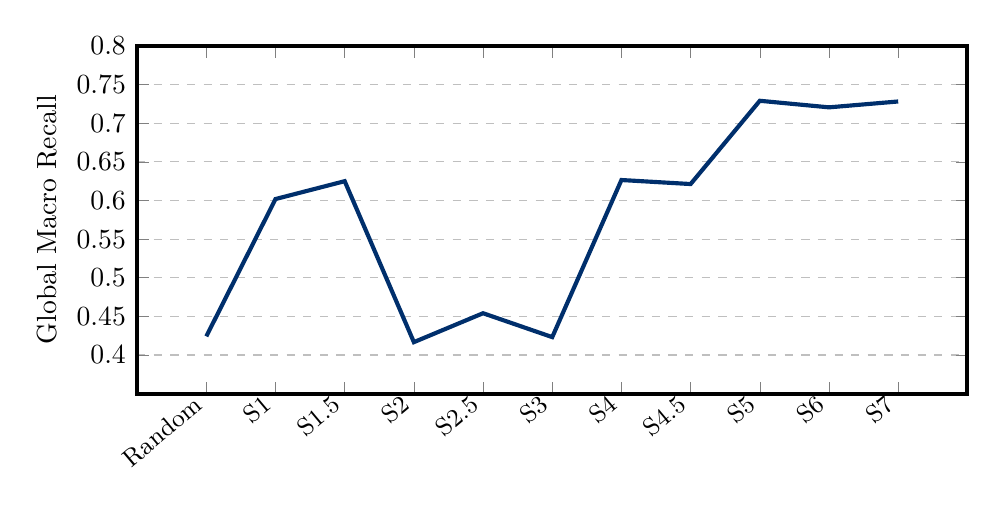
\begin{tikzpicture}
  \begin{axis}[
    width=\linewidth, height=6cm,
    ylabel={Global Macro Recall},
    symbolic x coords={Random,S1,S1.5,S2,S2.5,S3,S4,S4.5,S5,S6,S7},
    xtick=data,
    xticklabel style={rotate=40, anchor=east, font=\small},
    ymin=0.35, ymax=0.80,
    ytick={0.40,0.45,0.50,0.55,0.60,0.65,0.70,0.75,0.80},
    ymajorgrids=true, grid style=dashed,
    mark=*, mark size=2pt,
    line width=1.5pt,
  ]
  \addplot[color=iitblue] coordinates {
    (Random,0.4242)(S1,0.6018)(S1.5,0.6249)(S2,0.4167)(S2.5,0.4541)
    (S3,0.4232)(S4,0.6264)(S4.5,0.6212)(S5,0.7289)(S6,0.7204)(S7,0.7280)
  };
  \end{axis}
  \end{tikzpicture}
  \caption{Global Macro Recall progression across all strategies. Notable drops at S2 (full fine-tuning) and S3 (monolingual partitioning); decisive jump at S5 (generative SFT).}
  \label{fig:progression}
\end{figure}

\textbf{Phase analysis.} Three distinct phases emerged: (1) \emph{Feature extraction} (S1--S1.5, best: 0.6249) — frozen encoders excel on tiny datasets; (2) \emph{Discriminative fine-tuning} (S2--S4.5, plateau: $\sim$0.63) — data scarcity limits all fine-tuning paradigms; (3) \emph{Generative SFT} (S5--S7, best: 0.7289) — reasoning-as-generation breaks the plateau.

\textbf{S5 vs S7 complementarity.} S5 excels at \texttt{at} (0.6872); S7 excels at \texttt{isAt} (0.7817). An ensemble capturing the best of both is the most promising immediate direction.

%%==========================================================================
\section{Limitations}
%%==========================================================================

\begin{enumerate}
  \item \textbf{Data scarcity}: 104 gold documents across 3 languages and 3 label classes is the fundamental bottleneck. The binding constraint for fine-tuning approaches throughout.
  \item \textbf{PROBABLE class}: Systematically the hardest label across all strategies. Its inherent ambiguity resists both discriminative and generative approaches.
  \item \textbf{Multilingual gradient interference}: Mixing archaic DE/FR/EN in tiny batches creates destructive gradient updates (demonstrated empirically in S2--S3).
  \item \textbf{Multi-agent latency}: S7 requires $\sim$30 min for 21 documents on 3 GPUs, making it operationally expensive at test-set scale.
  \item \textbf{Wikidata gaps}: The death-date hard rule fires only when QIDs and biographical data are available — coverage is incomplete for many historical figures.
\end{enumerate}

%%==========================================================================
\section{Future Prospects}
%%==========================================================================

\begin{enumerate}
  \item \textbf{S5 + S7 Ensemble}: Majority voting or confidence-weighted fusion of complementary sub-task strengths; expected to push Global MR past 0.74.
  \item \textbf{Curriculum training}: Train specialists first on easy/unambiguous cases, then on PROBABLE cases to prevent early noisy gradient loss.
  \item \textbf{Self-consistency decoding}: Multiple reasoning chains per agent with majority-vote prediction to reduce single-sample variance.
  \item \textbf{RAG-Augmented Agents}: Historian with external biographical knowledge base; Geographer with historical gazetteer.
  \item \textbf{Iterative Debate}: Allow Historian and Geographer to observe each other's reasoning before the Arbiter synthesises.
  \item \textbf{Domain-adaptive pretraining}: Continued MLM on silver sandbox corpus to adapt vocabulary to historical OCR before SFT.
\end{enumerate}

%%==========================================================================
\section{Conclusion}
%%==========================================================================

We presented Team Hansel \& Gretel's complete experimental journey through nine strategies for Person--Place Relation Extraction in multilingual historical documents. The central finding is that \textbf{temporal reasoning in historical text cannot be reliably solved by discriminative classifiers alone}: generative models producing reasoning chains before their final labels substantially outperform classification heads (+9.45 points), even with smaller parameter counts. The multi-agent decomposition further demonstrates that specialised temporal and spatial reasoning perspectives are especially effective for the temporally-constrained \texttt{isAt} sub-task. Our best system (S5, Global MR $= 0.7289$) and final submission (S9, Wikidata-augmented CoT via GPT-OSS 120B) represent complementary approaches: one optimised for accuracy, the other combining scale with structured knowledge injection.

\begin{acknowledgments}
We sincerely thank the \textbf{HIPE-2026 organising team} --- Juri Opitz, Maud Ehrmann, Simon Clematide, Corina Racl\'{e}, Emanuela Boros, Andrianos Michail, and Matteo Romanello --- for the exceptional quality of the task design, data, and evaluation infrastructure. HIPE-2026 is organised within the framework of the Impresso -- Media Monitoring of the Past project (Swiss NSF grant No.~CRSII5\_213585; Luxembourg NRF grant No.~17498891). We also thank the \textbf{IBM Research RITS team} for API access to Llama 3.3 70B, Llama 4 Maverick, Granite 3.2 8B, and GPT-OSS 120B, which enabled Strategies 8 and 9.
\end{acknowledgments}

\section*{Declaration on Generative AI}
During the preparation of this work, the authors used AI-assisted coding tools for code generation and debugging assistance. All experimental results, analysis, and written content were reviewed and verified by the authors, who take full responsibility for the publication's content.

\bibliography{references}

\end{document}
